\chapter{Metodología}
\label{cap:metodologia}
En este capítulo se explicará todo lo relacionado con la metodología utilizada en este Trabajo Fin de Grado. Con el objetivo de encontrar una solución sostenible, flexible en términos de negocio y que sea capaz de amoldarse a las especificaciones y criterios del proyecto.\\

En primer lugar, se realizará una introducción a los equipos utilizados en el proyecto tanto a nivel software como hardware. Se detallarán las especificaciones técnicas y características de los equipos, así como su motivación para ser usados en este proyecto. De la misma manera se explicará el funcionamiento del software de configuración disponible en los equipos.\\

En segundo lugar, se realizarán pruebas a nivel de laboratorio utilizando configuraciones similares a las utilizadas en el marco del proyecto Napo. Siguiendo un escenario base de laboratorio, se analizará el rendimiento de los equipos a nivel de red, utilizando para ello herramientas cuya funcionalidad será la inyección de tráfico simulado. De forma paralela se utilizará la solución propuesta en el Capítulo \ref{cap:marco_teorico} para realizar la gestión y monitorización de redes sobre el escenario red disponible en laboratorio.

\section{Equipos propuestos}
Con el objeto de seleccionar aquellos equipos que mejor rendimiento y prestaciones ofrezcan al proyecto, se ha establecido una comparativa y estudio entre diferentes propuestas. Dichas propuestas no sólo deben adaptarse y cumplir a los requerimientos técnicos del proyecto, sino que también deben entrar en presupuesto, lo que limita de forma importante las opciones.\\

Para ello, primeramente se ha hecho una identificación de equipos que tuvieran las características buscadas, cuyo precio estuviera dentro de la gama de precios elegible y que estuvieran homologados para su despliegue en instalaciones reales en Perú. Con los equipos preseleccionados, se ha establecido un protocolo de pruebas que nos ofrecerá el rendimiento de los equipos sobre pruebas realizadas en campo; la batería de pruebas ha sido co-diseñada junto con el Grupo de Telecomunicaciones Rurales (GTR) de PUCP, y las pruebas se han ejecutado sobre un enlace largo en Lima, Perú, por parte del personal técnico del GTR. Dichas pruebas determinarán qué equipos son los finalmente seleccionados como solución del proyecto. A continuación, se procede a detallar cada uno de los equipos involucrados en este estudio y la comparativa entre ellos.

\subsection{Equipos Ubiquiti}
Los equipos de  comunicaciones inalámbricas de la empresa estadounidense Ubiquiti Networks \cite{Ubiquiti} son exportados y utilizados a lo largo de todo el mundo, convirtiendo así a la empresa en un referente mundial. Esta empresa se dedica principalmente al desarrollo y comercialización de dispositivos para redes inalámbricas, ya sean de larga o corta distancia. \\

Los equipos desarrollados por la empresa se caracterizan por su alto rendimiento, su bajo coste y su alta eficiencia energética, cmpliendo así con los requisitos mínimos establecidos en el proyecto Napo. En el marco del proyecto los equipos Ubiquiti AirFiber AF-5X y PowerBeam 5AC-620, los cuales se detallarán a continuación, han sido propuestos como solución. De igual forma, se ha detallado el \textit{software} de gestión de los equipos Ubiquiti, que en el caso de ambos funciona de idéntica forma.

\subsubsection{AirFiber AF-5X}
Los dispositivos AF-5x están diseñados con una carcasa de silicona que recubre la placa empotrada que forma el equipo, tal y como se muestra en la Figura \ref{af_5x}, el diseño sencillo de los equipos y sus conexiones salientes hacen de él un equipo muy versátil y flexible a la hora de ser integrado con otros componentes, como por ejemplo una antena o un sistema empotrado sobre una torre. Aparte de su flexibilidad a nivel físico, también ofrece gran versatilidad en su comportamiento, permitiendo así utilizar este equipo en diferentes roles según requiera la arquitectura diseñada, ya sea bien como estación base, o como un repetidor. De igual forma, su sistema está diseñado para ofrecer el máximo rendimiento de la transmisión mediante la reducción de señales interferentes y habilitando la posibilidad de utilizar constelaciones mayores para obtener un mayor \textit{throughput}.

\begin{figure}[H]
		\centering
		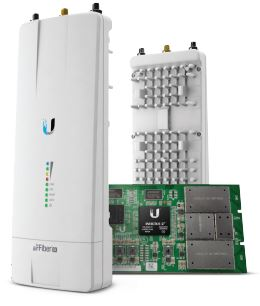
\includegraphics[width=5cm,height=5cm]{img/af_5x.JPG}
		\caption{Dispositivo AF-5X. Fuente: Ubiquiti Networks}
		\label{af_5x}
	\end{figure}

 Los dispositivos radio de esta familia, utilizan la banda de 5 GHz como frecuencia operacional y no sólo eso, si no que además este modelo abarca todo el espectro radioeléctrico en el rango de 5 GHz, tanto las bandas licenciadas como las que no lo son. Aparte de esto, estos equipos permiten ajustar el ancho de banda operacional, en el caso del modelo AF-5X de 10 a 50 MHz en intervalos de 10 MHz, otorgando mayor flexibilidad a la configuración de canales de subida y de bajada. Además de esto, los equipos permiten ajustar los canales de transmisión y recepción evitando así que existan interferencias en los canales seleccionados.
	
\subsubsection{PowerBeam 5AC-620}
La familia de equipos PowerBeam, independientemente del modelo, se caracteriza por su estructura y diseño, ya que tal y como se muestra en la Figura \ref{powerBeam} el dispositivo radio está integrado junto a la estructura de la parabólica, proporcionando así un mejor acople ya que se evitan las pérdidas con cable. Además esta característica en el diseño, los equipos PowerBeam cuentan con la tecnologías AirMAX AC desarrollada por Ubiquiti que permite focalizar la comunicación en una única dirección ofreciendo así robustez frente a interferencias filtrando el ruido no deseado.

\begin{figure}[H]
		\centering
		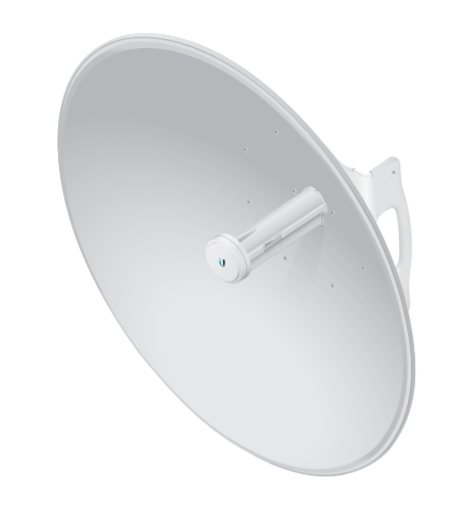
\includegraphics[width=5cm,height=5cm]{img/powerbeam.PNG}
		\caption{Dispositivo PowerBeam 5AC-620. Fuente: Ubiquiti Networks}
		\label{powerBeam}
\end{figure}

Otra característica importante de estos equipos es cómo permiten a los usuarios utilizar los enlaces para subida y descarga de datos. En este caso, la tecnologías AirMAX utiliza el protocolo de acceso al medio TDMA pero con una modificación desarrollada por Ubiquiti, ilustrado en la Figura \ref{tdma_ac}. Esta modificación consiste en asignar previamente \textit{slots} de tiempo a los usuarios mediante un punto de acceso inteligente integrado en el propio dispositivo, esto permite minimizar problemas de colisión cómo el problema del nodo escondido y aumentar el rendimiento del equipo llegando a obtener tasas mayores a 450 Mbps mientras que los equipos sin dicha tecnologías se mantienen en el umbral de 150 Mbps.
	
\begin{figure}[H]
		\centering
		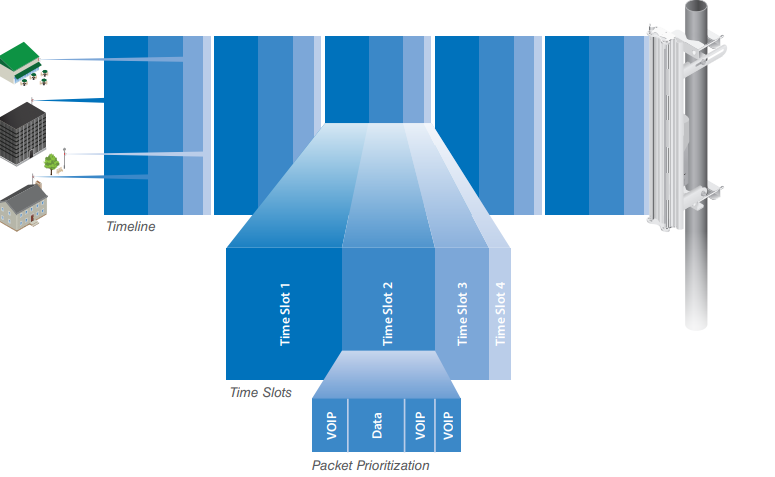
\includegraphics[width=0.5\textwidth]{img/tdma_ac.PNG}
		\caption{Protocolo TDMA con tecnologías AirMAX AC. Fuente: Ubiquiti Networks}
		\label{tdma_ac}
\end{figure}
	
\subsection{Software}
Los equipos propietarios de la marca Ubiquiti utilizan un \textit{software} propietario que permite controlar y configurar los equipos. Aunque no esté en su versión final, el programa Ubiquiti Network Management System (UNMS) otorga al usuario un control absoluto sobre los dispositivos que conforman la red, y una serie de aplicaciones internas para obtener una correcta parametrización del rendimiento de los equipos. Tal y como se muestra en la Figura \ref{unms} podemos ver como la pantalla principal del \textit{software} muestra diferentes tipos de configuración, paneles de interacción con el usuario, así como diferentes pestañas en las cuales se muestran datos a tiempo real del rendimiento de los equipos. 

\begin{figure}[H]
		\centering
		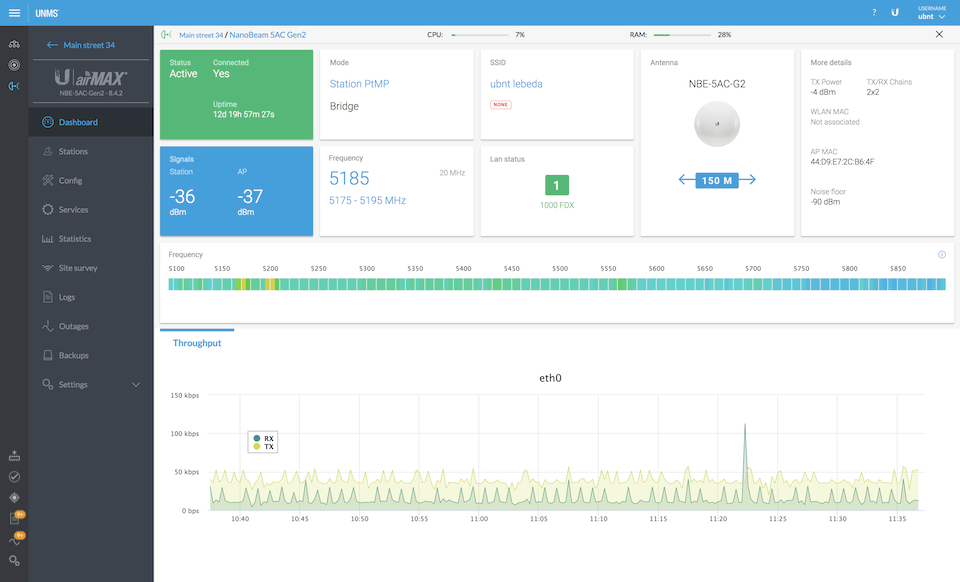
\includegraphics[width=0.5\textwidth]{img/unms.png}
		\caption{Pantalla principal UNMS. Fuente: Ubiquiti Networks}
		\label{unms}
	\end{figure}
	
Aparte de las funcionalidades antes comentadas, UNMS ofrece la posibilidad de obtener datos referentes al rendimiento de los equipos en lo que a parametrización de red respecta, es decir, todo lo relacionado con tráfico entrante y saliente de la red, niveles de recepción de señal, etc... Dichos parámetros pueden obtenerse utilizando una apicación interna que la propia herramienta tiene integrada consigo.

\subsection{Equipos VNL: RM-MAX}
Los equipos inalámbricos RM-MAX son fabricados y comercializados por la empresa VNL \cite{VNL}. Fundada en 2004, VNL se dedica al desarrollo e implementación de equipos para infraestructuras de telecomunicaciones punto a punto. Aunque su principal enfoque estratégico sea en aplicaciones militares y civiles, actualmente existe una creciente demanda de uso de estos equipos en zonas rurales de países en vías de desarrollo, como por ejemplo India, Nepal o Indonesia.\\

Los equipos RM-MAX  utilizan OFDM como protocolo de acceso al medio, pero este procotocolo no es el nativo, es decir, es una variante propietaria de VNL que permite mantener las conexiones existentes de forma prolongada evitando caídas con la parte \textit{core} de la red. De igual forma, los equipos permiten un control absoluto sobre las transmisiones existentes en la red, consiguiendo así una reducción en costes importante evitando el uso de líneas cableadas. Otro factor a tener en cuenta, es que dichos equipos están fabricados y desarrollados bajo la metodología \textit{Plug and Play}, lo que quiere decir que su instalación y configuración se realiza forma rápida y sencilla.

\subsubsection{Hardware}
Los equipos RM-MAX escogidos como solución de este proyecto, nominalmente son capaces de cubrir una distancia superior a los 100 Km incluyendo diferentes configuraciones según la frecuencia que deseemos usar. Tal y como se muestra en la Figura \ref{rm_max}, la antena está integrada en una placa cuyo recubrimiento metálico hace que este equipo sea robusto frente a situaciones climatólogicas adversas. De igual forma dichos equipos están dotados de diferentes modos de funcionamiento, lo que permite mayor versatilidad a lo hora de configurar un tipo determinado de infraestructura, de igual forma estos equipos admiten diferentes modos de actuación, ya sea bien como estación base o como \textit{bridge}.

\begin{figure}[H]
		\centering
		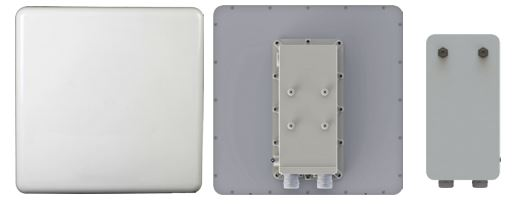
\includegraphics[width=0.5\textwidth]{img/rm_max.JPG}
		\caption{Dispositivo RM-MAX. Fuente: Vihaan Networks limited}
		\label{rm_max}
	\end{figure}
	
\subsubsection{Software}
Los equipos VNL utilizan como \textit{software} de gestión y configuración el \textit{Radio Modem Management}, dicho programa es propietario de VNL y muestra un aspecto similar al que se muestra en la Figura \ref{vnl_rm}. Dicha aplicación permite configurar de manera sencilla los parámetros de red deseables en cuanto a configuración se refiere, obteniendo así un escenario versátil y fácilmente gestionable. De igual forma, la aplicación nos permite configurar perfiles de seguridad y administración para atribuir mayor robustez a la red configurada. 

\begin{figure}[H]
		\centering
		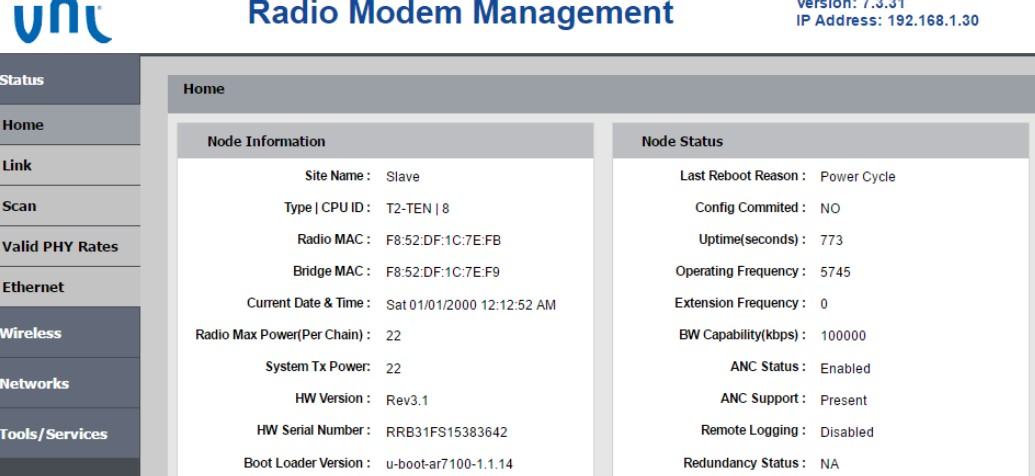
\includegraphics[width=0.5\textwidth]{img/vnl_rm.jpg}
		\caption{Pantalla principal \textit{Radio Modem Management}. Fuente: Vihaan Networks limited}
		\label{vnl_rm}
	\end{figure}

Por otra parte, la aplicación ofrece la posibilidad de configurar páginas de entrada por el usuario, permitiendo así una mayor personalización de la herramienta en función del perfil del usuario. Esta funcionalidad permite al usuario obtener datos en tiempo real del estado y actuación de los equipos involucrados en la red. 

\subsection{Equipos Mikrotik: NetMetal 5}
Los equipos NetMetal 5 son dispositivos pertenecientes a la familia de RouterBOARD diseñadas y comercializadas por la empresa MikroTik \cite{Mikrotik}. Dicha empresa se dedica al desarrollo de sistemas hardware y software inalámbricos. El uso de sus equipos está extendido a nivel mundial debido a su bajo coste y a su alto rendimiento en sistemas de telecomunicaciones inalámbricas.
	\subsubsection{Hardware}
	Los equipos NetMetal disponen de un procesador MIPSBE que opera a 720MHz y un recubrimiento hecho de aluminio y metal, su aspecto se muestra en la Figura \ref{equipo}, lo que permite un gran rendimiento en zonas donde existen condiciones climatológicas adversas. El equipo está formado por tres puertos cuya funcionalidad es: la conexión de antenas externas en dos de ellos (permitiendo el uso de MIMO), y un terminal POE en el que se encuentran las entradas para la conexión mediante ethernet y la fuente de alimentación.
	\begin{figure}[H]
		\centering
		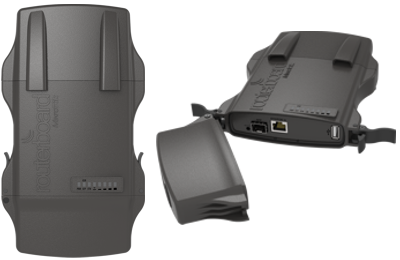
\includegraphics[width=0.5\textwidth]{img/netMetal5.png}
		\caption{Dispositivo NetMetal 5. Fuente: Mikrotik Router and Wireless}
		\label{equipo}
	\end{figure}
	Existe una variante en los equipos, el cual en vez de proporcionar tres entradas para antenas externas únicamente proporciona dos entradas.
	Los equipos NetMetal 5 son capaces de alcanzar altas tasas de transmisión en comunicaciones inalámbricas de larga distancia, gracias al uso del estándar 802.11ac y su eficiencia en cuanto al uso de los canales de 20/40/80 MHz. Este hecho añadido a su robustez hacen de los equipos una elección idónea para el contexto del proyecto.
	
	
	
	\subsubsection{Software}
	El sistema operativo que utilizan los equipos es RouterOS, propietario de MikroTik. Dicha distribución nos permite acceder al dispositivo de manera sencilla y configurar el equipo acorde al escenario requerido. Además de realizar configuraciones en cuánto a los parámetros deseados, el sistema operativo ofrece herramientas para la realización de pruebas a diferentes niveles de conectividad entre equipos. Los datos obtenidos, pueden ser procesados y representados de forma gráfica en tablas, diagramas y ficheros de texto. Independientemente de un formato u otro existe la posibilidad de exportar estos datos.\\
	
	Así mismo los equipos permiten exportar e importar las configuraciones realizadas siendo esto de gran utilidad a la hora de replicar una configuración en diferentes equipos. Por último este sistema operativo es compatible con cualquier distribución para PC, ofrece más de una variante para utilizar y configurar los equipos, ya sea mediante línea de comandos, interfaz web o utilizando la aplicación WinBox que se detalla a continuación.\\
	
	WinBox permite conectar los equipos de manera rápida y sencilla a través de su dirección IP o MAC, tal y como se muestra la siguiente Figura \ref{inicioWinBox}. La configuración de usuario e IP vienen predeterminadas por el fabricante.\\
	
	Una vez logueado dentro del equipo, tal y como se muestra en la Figura \ref{mainWinBox}, aparecen multitud de paneles y menús los cuales nos servirán para configurar los equipos, ya sea en cuestiones de seguridad, creación de redes, configuración de interfaces, etc... Aparte de modificar la configuración que se establece predeterminada, WinBox ofrece la posibilidad de realizar mediciones para determinar el rendimiento de los equipos, como por ejemplo el número de paquetes envíado durante una transmisión.
		\begin{figure}[H]
			\centering
			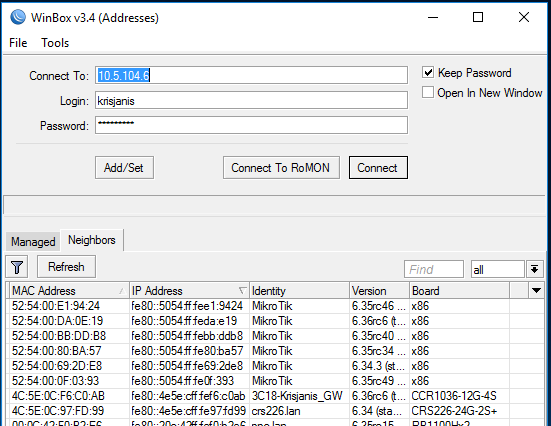
\includegraphics[width=0.7\textwidth]{img/winbox_loader.png}
			\caption{Pantalla loging en WinBox. Fuente: Mikrotik Router and Wireless}
			\label{inicioWinBox}
		\end{figure}
		\begin{figure}[H]
			\centering
			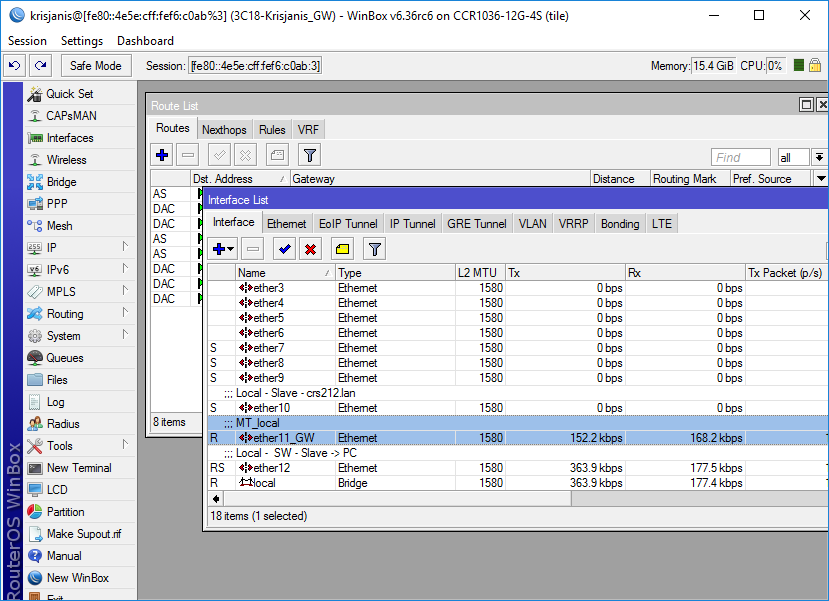
\includegraphics[width=0.7\textwidth]{img/winbox.png}
			\caption{Pantalla principal en WinBox. Fuente: Mikrotik Router and Wireless}
			\label{mainWinBox}
		\end{figure}
		Al igual que la herramienta web, WinBox ofrece la posibilidad de utilizar una terminal compatible con el equipo y sistema operativo RouterOS. Dicha funcionalidad permite introducir y modificar las configuraciones existentes en los dispositivos, así cómo visualización de parámetros y realización de pruebas utilizando las herramientas integradas que posee el sistema operativo.\\
		
			Además de lo comentado anteriormente, otra característica importante que poseen estos equipos es su protocolo inalámbrico Nstreme. Nstreme es un protocolo propietario de Mikrotik cuya versión más reciente es NV2, la cual basa su funcionamiento en TDMA. Este protocolo es soportado por cualquier \textit{hardware} relacionado con el protocolo 802.11 siendo posible así la interoperabilidad entre equipos en una misma red. Por un lado, para realizar una correcta gestión del acesso al medio, el NV2 \textit{access point} divide el tiempo en períodos de tamaño fijo, que son dinamicamente asignados para \textit{uplink} y \textit{downlink} en función del estado de colas en el \textit{access point} y los clientes.  Por otro lado, parte de ese tiempo es destinado a "nuevos clientes" que desean conectarse a la red y aprovechan para realizar el registro y primer intercambio de datos con el \textit{access point}. Nv2 no restringe el uso de tasa entre los clientes que forman la red, permitiendo así una comunicación confiable entre los miembros de la misma.
			
\section{Planificación e instalación de la red}
Una vez detallado y estudiado las principales características de los equipos candidatos a solución del proyecto, es importante definir cuales van a ser los criterios y pruebas a los que serán sometidos los equipos para elegir aquel que será solución del proyecto. \\

En primer lugar para poder conocer la viabilidad y calidad de enlace en cuanto al uso de los equipos, trazaremos perfiles simulados con la herramienta RadioMobile que nos servirá para realizar una primera aproximación sobre la viabilidad del enlace y además, podremos comparar los resultados obtenidos mediante la simulación ya que el escenario de pruebas será el mismo para todos los equipos. Dicho escenario ha sido propuesto por los compañeros de la PUCP, el cual además de realizarse de forma teórica se aplicará de forma práctica pudiendo contrastar entre las prestaciones de los equipos en ambas situaciones, por último se escogerá uno de los equipos como solución y se replicará el escenario en laboratorio. \\

En paralelo a las pruebas de los equipos, realizaremos un estudio teórico basándonos en los datos extraídos del artículo \cite{simo2014assessing} referente al protocolo inalámbrico NV2. En este caso las pruebas que se realizaron con una parámetros de enlace distintos a los definidos en el proyecto Napo, no obstante dichas mediciones y valores obtenidos pueden ser extrapolables en lo que a nuestros contexto se refiere. Para ello realizaremos un desarrollo analitico de los resultado, los cuales serñan representados en gráficas, y obtendremos de forma aproximada el rendimiento que debemos de esperar de los equipos que utilicen el protocolo NV2. \\

En segundo lugar se configurará un escenario similar al proporcionado por los compañeros de la PUCP en laboratorio. Dicho escenario estará compuesto por dos terminales pc y dos equipos de los elegidos como solución que estarán interconectados de forma que sea posible la comunicación punto a punto. Una vez configurada esta red, el siguiente paso será realizar pruebas respecto al tráfico utiliza programas de inyección de tráfico para conocer el rendimiento de los equipos y conocer los límites en cada radioenlace.\\

Por último se integrará dicho escenario con el \textit{software} de monitorización escogido para tal efecto, pero antes de eso, se realizará un breve introducción a la monitorización y gestión de redes, detallando los principales protocolos involucrados en la capa de aplicación. A continuación, se mostrarán diferentes configuraciones aplicables sobre el escenario real de la red que permiten a cualquier usuario obtener un control total sobre la misma.

